\documentclass[unknownkeysallowed]{beamer}
\usepackage[french,english]{babel}
\usepackage{pythontex}
\usepackage[francais]{babel}
\usepackage{xcolor}
\usepackage{movie15}
\usepackage[utf8]{inputenc}
\usepackage{pythontex}
\usepackage{fontawesome}
\usetheme{Madrid}
\usecolortheme{beaver}
\usepackage{utopia}%font utopia imported
\usepackage{graphicx}
\newtheorem{exmp}{Exemple}[section]
\usetheme{Boadilla}
\usecolortheme{beaver}
\renewcommand{\contentsname}{Table des matières} 

\begin{document}


%%%%%%%%%%%%%%%%%%%%%%%%%%%%%%%%%%%%%%%%%%%%%%%%%%%%%%%%%%%%%%%%%%%%%%%%%%%%%%%
%%%%%%%%%%%%%%%%%%%%%%             Headers               %%%%%%%%%%%%%%%%%%%%%%
%%%%%%%%%%%%%%%%%%%%%%%%%%%%%%%%%%%%%%%%%%%%%%%%%%%%%%%%%%%%%%%%%%%%%%%%%%%%%%%



%%%%%%%%%%%%%%%%%%%%%%%%%%%%%%%%%%%%%%%%%%%%%%%%%%%%%%%%%%%%%%%%%%%%%%%%%%%%%%%
\begin{frame}
\bigskip
\bigskip
\begin{center}{
\LARGE\color{marron}
\textbf{HMMA 307 : Advanced Linear Modeling}
\textbf{ }\\
\vspace{0.5cm}
}

\color{marron}
\textbf{Chapter 1 : Linear regression}
\end{center}

\vspace{0.5cm}

\begin{center}
\textbf{Emma Santinelli \ Mégane Diéval \ Yassine Sayd} \\
\vspace{0.1cm}
\url{https://github.com/MegDie/advanced_lm_introduction}\\
\vspace{0.5cm}
Université de Montpellier \\
\end{center}

\centering

\includegraphics[width=0.13\textwidth]{umontpellier_logo}
\end{frame}
%%%%%%%%%%%%%%%%%%%%%%%%%%%%%%%%%%%%%%%%%%%%%%%%%%%%%%%%%%%%%%%%%%%%%%%%%%%%%%%
%%%%%%%%%%%%%%%%%%%%%%%%%%%%%%%%%%%%%%%%%%%%%%%%%%%%%%%%%%%%%%%%%%%%%%%%%%%%%%%
%%%%%%%%%%%%%%%%%%%%%%%%       PLAN      %%%%%%%%%%%%%%%%%%%%%%%%%%%%%%%%%%%%%%
%%%%%%%%%%%%%%%%%%%%%%%%%%%%%%%%%%%%%%%%%%%%%%%%%%%%%%%%%%%%%%%%%%%%%%%%%%%%%%%


%%%%%%%%%%%%%%%%%%%%%%%%%%%%%%%%%%%%%%%%%%%%%%%%%%%%%%%%%%%%%%%%%%%%%%%%%%%%%%%
\begin{frame}{Table of Contents}
\tableofcontents[hideallsubsections]
\end{frame}
%%%%%%%%%%%%%%%%%%%%%%%%%%%%%%%%%%%%%%%%%%%%%%%%%%%%%%%%%%%%%%%%%%%%%%%%%%%%%%%



%%%%%%%%%%%%%%%%%%%%%%%%%%%%%%%%%%%%%%%%%%%%%%%%%%%%%%%%%%%%%%%%%%%%%%%%%%%%%%%
\AtBeginSection[]
{
\begin{frame}<beamer>{Table of Contents}
\tableofcontents[currentsubsection,
    hideothersubsections,
    sectionstyle=show/shaded,
]
\end{frame}
}
%%%%%%%%%%%%%%%%%%%%%%%%%%%%%%%%%%%%%%%%%%%%%%%%%%%%%%%%%%%%%%%%%%%%%%%%%%%%%%%




%%%%%%%%%%%%%%%%%%%%%%%%%%%%%%%%%%%%%%%%%%%%%%%%%%%%%%%%%%%%%%%%%%%%%%%%%%%%%%%
%%%%%%%%%%%%%%%%%%%%%%%%%%%%%%%%%%%%%%%%%%%%%%%%%%%%%%%%%%%%%%%%%%%%%%%%%%%%%%%
\section{Introduction and Ordinary Least Squares}
\label{sec:introdcution}
%%%%%%%%%%%%%%%%%%%%%%%%%%%%%%%%%%%%%%%%%%%%%%%%%%%%%%%%%%%%%%%%%%%%%%%%%%%%%%
%%%%%%%%%%%%%%%%%%%%%%%%%%%%%%%%%%%%%%%%%%%%%%%%%%%%%%%%%%%%%%%%%%%%%%%%%%%%%%%

%%%%%%%%%%%%%%%%%%%%%%%%%%%%%%%%%%%%%%%%%%%%%%%%%%%%%%%%%%%%%%%%%%%%%%%%%%%%%%%

%%%%%%%%%%%%%%%%%%%%%%%%%%%%%%%%%%%%%%%%%%%%%%%%%%%%%%%%%%%%%%%%%%%%%%%%%%%%%%%

%%%%%%%%%%%%%%%%%%%%%%%%%%%%%%%%%%%%%%%%%%%%%%%%%%%%%%%%%%%%%%%%%%%%%%%%%%%%%%%
\begin{frame}{Model}
Suppose the data consists of $n$ samples $( y_i, x_i )^n_{i=1}$ with $p$ features.
\newline The model can be written in matrix notation as :
\begin{center}
$y=X\beta+\varepsilon$
\end{center}
where
 \begin{itemize}
        \item $X$ is an $n$$\times$$p$ matrix of regressors
        \item $\beta$  is a $p$$\times$1 vector of unknown parameters
        \item $\varepsilon$ is a vector of normal random errors with mean 0
    \end{itemize}
\end{frame}
\begin{frame}
The OLS estimator is any coefficient vector
$\hat\beta^{\rm LS}\in\mathbb{R}^p$ such that :
\newline
\begin{center}
$\hat\beta^{\rm LS} \in \argmin_{\beta \in \bbR^p}
\underbrace{\frac{1}{2n}\|y-X\beta\|^2 }_{f(\beta)}$
\end{center}
\vspace{0.5cm}

and
\begin{align*}
	f(\beta)
	= \frac{1}{2n}\sum_{i=1}^n (y_{i}-\frac{1}{2n}(X\beta)_{i})^2
	= \beta^{\top}\frac{X^{\top}X}{2n}\beta+\frac{1}{2n}\|y\|^2- \langle y,X\beta\rangle
\end{align*}

\vspace{0.5cm}
where
$\langle y,X\beta\rangle=y^{\top}X\beta=\beta^{\top}X^{\top}y=\langle \beta,X^{\top}y\rangle$.
\end{frame}

\begin{frame}{The Gram matrix}


\begin{block}{Notation}
The matrix $\hat\Sigma=\frac{X^{\top}X}{n}$ matrix is called the Gram matrix.
\begin{center}
   $X^{\top}X=\begin{pmatrix}
   x_{1}^{\top}  \\
   \vdots   \\
   x_{p}^T  \\
\end{pmatrix}(x_{1},\dots, x_{p}) $,
\end{center}
\end{block}

The Gram matrix is equivalent to :

\begin{center}
$[X^{\top}X]_{j,j'}=[\langle x_{j},x_{j'}\rangle]_{(j,j')\in[1,p]^2}$ 
\end{center}


\end{frame}



\begin{block}{Remark}
Most of the times, we scale features.
\newline
We have : $\bar{X_{j}}=\frac{1}{n} \sum\limits_{i=1}^{n} x_{ij}$ (1).
\newline
 To center explanatory variables, we use the equation (1) to build the centered vector $X_{c}$.
\newline
$X_{c} = X - (\bar{X_{1}}1_n,\dots,\bar{X_{p}}1_n)$ where $\1_n=(1,\dots,1)$.

Then we obtain $\bar{X_{c}}=0_n$.

To reduce explanatory variables, we use :
\newline
\begin{center}
$\hat\sigma_{j}^2=\frac{1}{n} \sum\limits_{i=1}^{n} (X_{ij}-\bar{X_{j}})$
\end{center}
Let $X_r$ be the reduced vector, then :
\newline
\begin{center}
$X_{r_{j}}=\frac{X_{j}-\bar{X_{j}}1_n}{\hat\sigma_{j}}$    
\end{center}

\end{block}


\begin{frame}
\begin{alertblock}{First Order Optimality Conditions}
We can verify the first order optimality condition because $\nabla{f(\hat\beta^{\rm LS})}=0$
\\
Note that $f$ is a $C^{\infty}$ function, then differentiable

\end{alertblock}

\begin{block}{Remark}
\rem $f$ is a convex function so a local minimum is a global one.
\end{block}

\begin{block}{Conclusion}
$\hat\beta^{\rm LS}$ satisfy the following equations of orthogonality :
\begin{itemize}
         \item $\frac{X^{\top}X}{n}\hat\beta^{\rm LS}-\frac{X^{\top}y}{n}=0$
        \item $\iff X^{\top}(\frac{X\hat\beta^{\rm LS}-y}{n})=0$
        \item $\iff X^{\top}(y-X\hat\beta^{\rm LS})=0$
        \item $\iff \langle X_{j},y-X\beta\rangle=0$ for $j \in [1:p]$
    \end{itemize}


\end{block}

\newpage


\begin{block}{Warning!}
If $p < n$ so ${\rm rank}(X) \leq n < p$.Then, $\hat{\beta}^{\rm LS}$ is not unique.
\end{block}


\end{frame}

\begin{frame}

\begin{alertblock}{Interpretation}
    \begin{itemize}
        \item  Each explanatory feature is orthogonal to the residuals $\Gamma=y-X\hat{\beta}^{\rm LS}$ With $\hat{\beta}^{\rm LS}$ a solution of the linear $p$$\times$$p$ system : $$ \hat{\Sigma}\beta= \frac{X^{\top} y}{n}  $$

    \end{itemize}


\end{alertblock}

\begin{block}{Remarks}
    \begin{itemize}
        \item  If $\hat{\Sigma}$ is invertible, the solution of the linear system is unique
        \item $\hat{\Sigma}$ is invertible $\Rightarrow$ $\hat{\Sigma}$ is positive definite
        \item If $\hat{\Sigma}$ invertible, so $rank(\hat{\Sigma})=p$
        \item we assume that we have a full rank column e.g. : $$rank(X)=dim(Vect(X_1,...,X_p)) \leq n $$

    \end{itemize}


\end{block}
\end{frame}



\begin{frame}



\begin{alertblock}{Remark}
    \begin{itemize}
        \item  If $rank(X)=p$, so $\hat{\Sigma}$ is invertible and : $$\hat{\beta}^{\rm LS}=\hat{\Sigma}^{-1}\frac{X^{\top} y}{n}=(\frac{X^{\top} y}{n})^{-1} \frac{X^{\top} y}{n}$$
       then :  $$ \hat{\beta}^{\rm LS}=(X^{\top}X)^{-1}X^{\top}y$$

    \end{itemize}


\end{alertblock}

\begin{block}{Notice}
    \begin{itemize}
        \item  In practice, it is exceptional to invert $\hat{\Sigma} $ because one solves many linear systems
       
    \end{itemize}


\end{block}
\end{frame}

\begin{frame}{Data analysis}

\begin{block}{Goal}
    We want to build some ordinary least squares models of prediction with two datasets:

    \begin{itemize}
          \item Bicycle accidents
          \item Count data of bicycles
      \end{itemize}
\end{block}

\vspace{0.5cm}

We propose to estimate the severity of accidents by the feature "sexe". The problem is that the features are qualitative:
\begin{itemize}
    \item Modalities of the feature to predict: "0 - Indemne", "1 - Blessé léger", "Blessé hospitalisé", and "3 - Tué"
    \item Modalities of the feature "sexe": "M" and "F"
\end{itemize}


\end{frame}

\begin{frame}{Data analysis}

\begin{alertblock}{Solution}
We convert features into ordinal features.
\end{alertblock}

\begin{block}{Prediction principle}

Calculate the coefficients $\beta$ on a training sample and predict on a test sample the feature of interest. 0 is the value for male and 1 is the value for female.

\end{block}

\begin{minipage}[c]{.36\linewidth}
     \begin{center}
             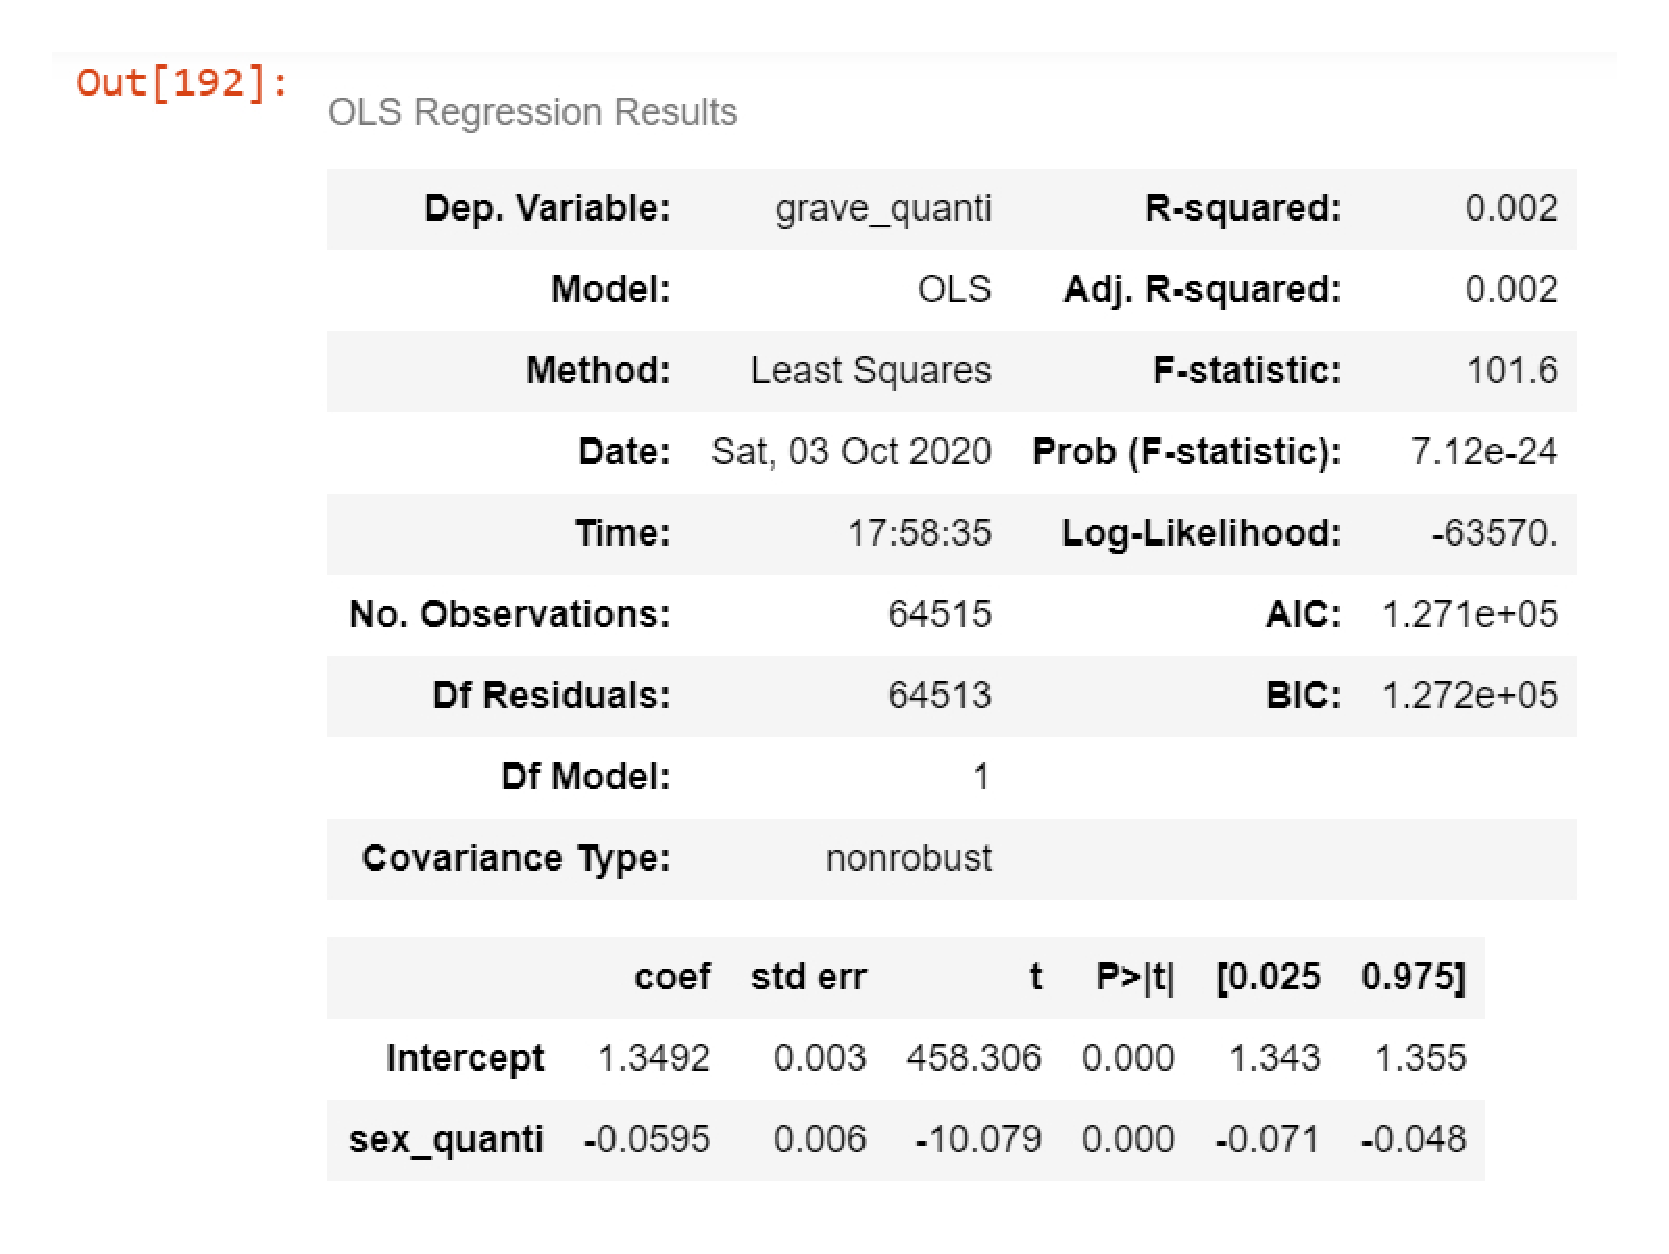
\includegraphics[width=5.5cm]{stat_model_gravity}
         \end{center}
   \end{minipage} \hfill
   \begin{minipage}[c]{.55\linewidth}
    \begin{center}
            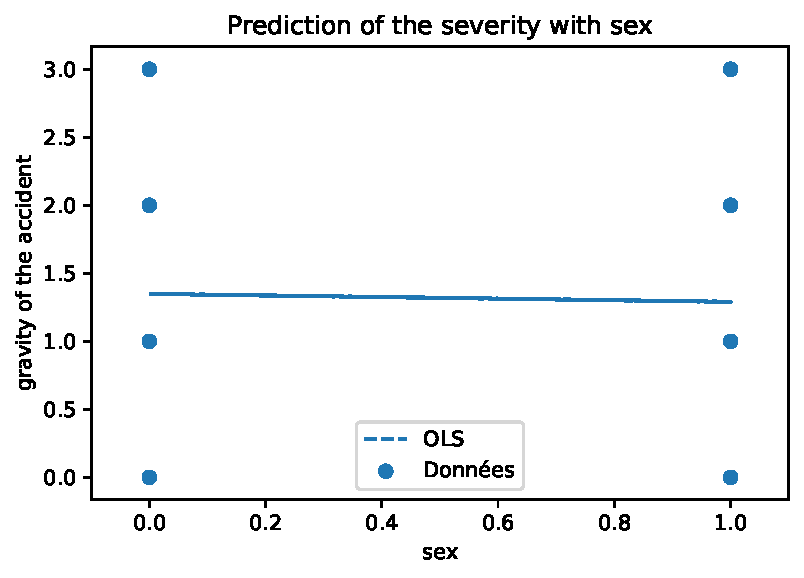
\includegraphics[width=5.5cm]{severitypredictionwithsex}
            
        \end{center}
  
 \end{minipage}

\end{frame}

\begin{frame}{Data analysis}

\begin{block}{Conclusion}
The prediction is very bad on qualitative features. We notice that the $R^2$ is closed to 0 and it's mostly the same with the others qualitative features. With this dataset, the OLS model is not efficient enough for qualitative features.

\end{block}

\begin{block}{Prediction of a quantitative feature}
Predict the number of accidents with the date (day, month and year) that is an ordinal feature with periodic component. Results are also very bad.

\end{block}

\begin{minipage}[c]{.36\linewidth}
     \begin{center}
             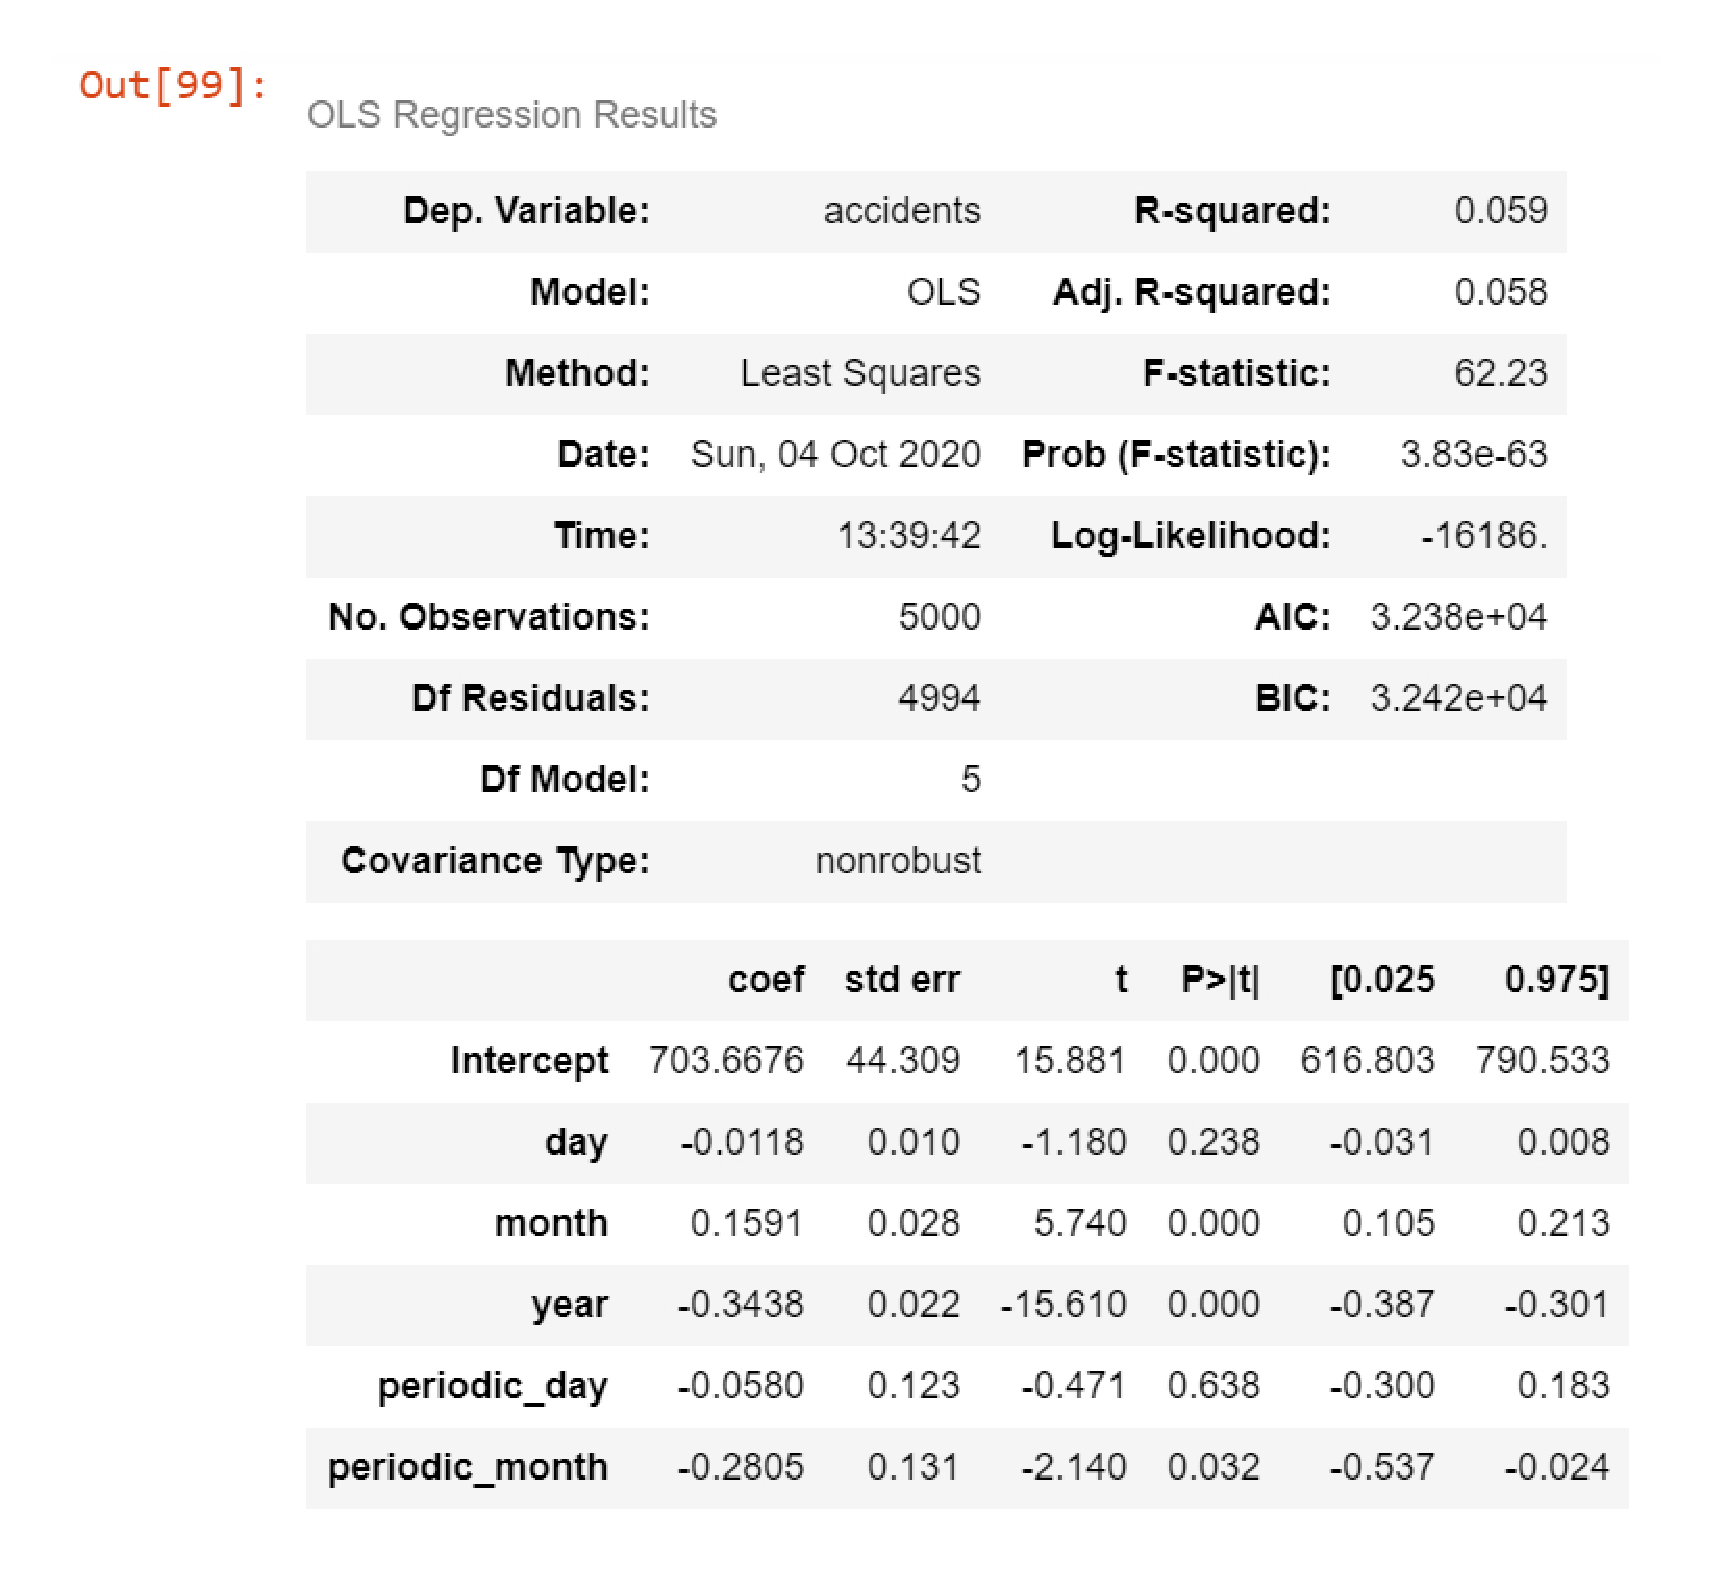
\includegraphics[width=4cm]{stat_model_number1}
         \end{center}
   \end{minipage} \hfill
   \begin{minipage}[c]{.55\linewidth}
    \begin{center}
            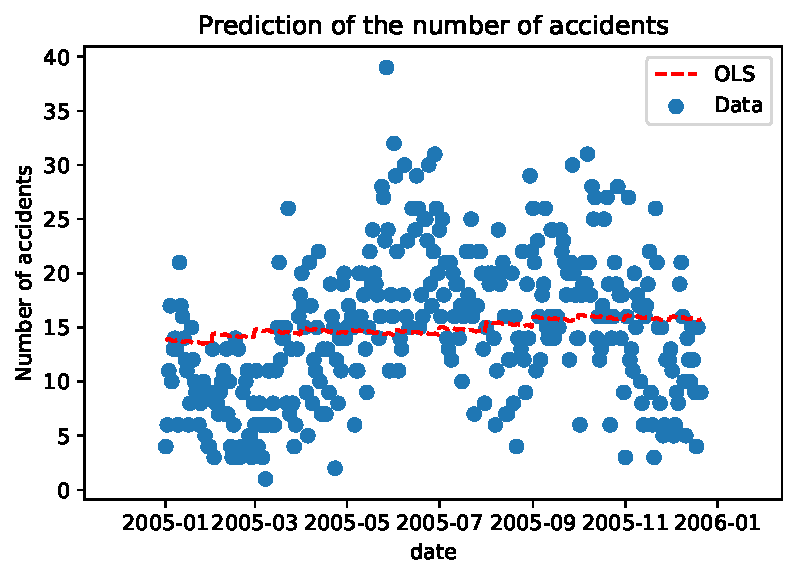
\includegraphics[width=5.5cm]{accidentprediction}
            
        \end{center}
 
 \end{minipage}

\end{frame}

\begin{frame}{Data analysis}

\begin{block}{Similar idea on the second dataset}
Prediction of the number of bicycles in a day with the date and the total number of bicycles. We introduce also periodic components.
\end{block}


\begin{minipage}[c]{.36\linewidth}
     \begin{center}
             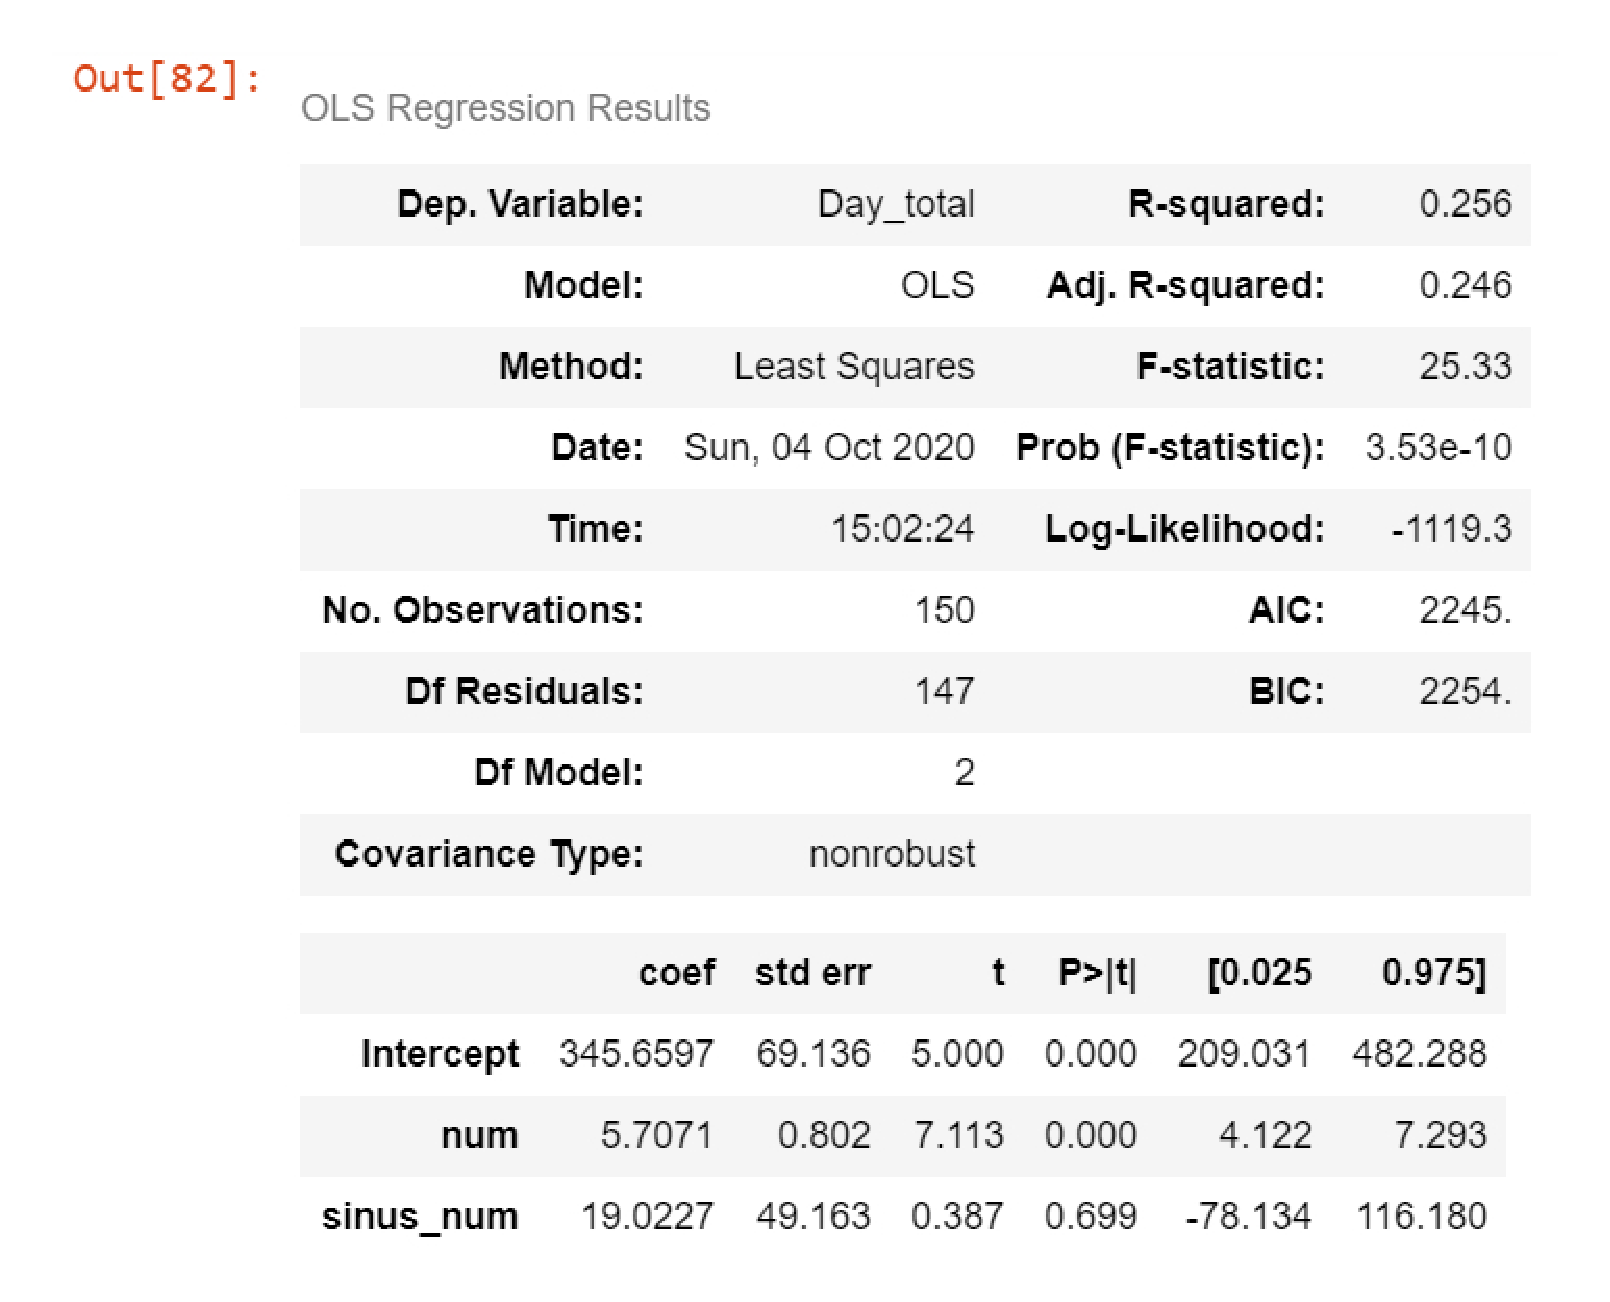
\includegraphics[width=4cm]{stat_model_albert}
         \end{center}
   \end{minipage} \hfill
   \begin{minipage}[c]{.55\linewidth}
    \begin{center}
            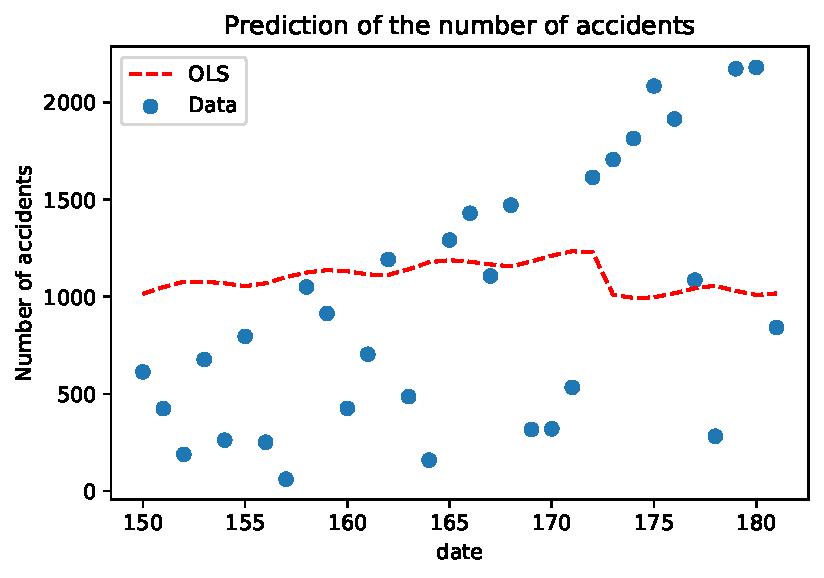
\includegraphics[width=5.5cm]{accidentpredictionalbert1}
            
        \end{center}

 \end{minipage}




\end{frame}





%%%%%%%%%%%%%%%%%%%%%%%%%%%%%%%%%%%%%%%%%%%%%%%%%%%%%%%%%%%%%%%%%%%%%%%%%%%%%%%



%%%%%%%%%%%%%%%%%%%%%%%%%%%%%%%%%%%%%%%%%%%%%%%%%%%
%%%%%%%%%%%%%%%%%%%%%%%%%%%%%%%%%%%%%%%%%%%%%%%%%%%%%%%%%%%%%%%%%%%%%%%%%%%%%%%



%%%%%%%%%%%%%%%%%%%%%%%%%%%%%%%%%%%%%%%%%%%%%%%%%%%%%%%%%%%%%%%%%%%%%%%%%%%%%%%

%%%%%%%%%%%%%%%%%%%%%%%%%%%%%%%%%%%%%%%%%%%%%%%%%%%%%%%%%%%%%%%%%%%%%%%%%%%%%%%
%%%%%%%%%%%%%%%%%%%%%%%%%%%%%%%%%%%%%%%%%%%%%%%%%%%%%%%%%%%%%%%%%%%%%%%%%%%%%%%
\section{Singular Value Decomposition}
\label{sec:conclusion}
%%%%%%%%%%%%%%%%%%%%%%%%%%%%%%%%%%%%%%%%%%%%%%%%%%%%%%%%%%%%%%%%%%%%%%%%%%%%%%%
%%%%%%%%%%%%%%%%%%%%%%%%%%%%%%%%%%%%%%%%%%%%%%%%%%%%%%%%%%%%%%%%%%%%%%%%%%%%%%%

\begin{frame}
\begin{block}{Reminder}
Let $\Sigma\in\mathbb{R}^{p \times p}$.
\newline
If $\Sigma^{\top}=\Sigma$ then $\Sigma$ is diagonalizable.
\end{block}
\begin{alertblock}{Theorem}
For all matrix $M\in\mathbb{R}^{m_1 \times m_2}$ of rank $r$, there exist two orthogonal matrix $U\in \mathbb{R}^{m_1 \times r}$ and $V\in\mathbb{R}^{m_2 \times r}$ such that :
\begin{center}
    $M=U \diag(s_{1},\dots, s_{r})U^{\top}$
\end{center}
where $s_{1}\ge s_{2} \ge ... \ge s_{r} \ge 0$ are the singular values of M.
\end{alertblock}
\vspace{0.5cm}
Note that : $M=\sum_{j=1}^r s_{j}u_{j}v_{j}^{\top}$ with : $U=[u_{1},\dots,u_{r}]$ and $V=[v_{1} \dots v_{r}]$.
\end{frame}
%%%%%%%%%%%%%%%%%%%%%%%%%%%%%%%%%%%%%%%%%%%%%%%%%%%%%%%%%%%%%%%%%%%%%%%%%%%%%%%

\begin{frame}
\begin{block}{Definition}
For $M\in\mathbb{R}^{m_1 \times m_2}$, a pseudoinverse of $M$ is defined as a matrix $M^{+}$ satisfying :
\begin{center}
    $M^{+}=Vdiag(\frac{1}{s_{1}} \dots \frac{1}{s_{r}})U^{\top}$
    =$\sum\limits_{j=1}^r \frac{1}{s_{j}}v_{j}u_{j}^{\top}$
\end{center}
\end{block}
\vspace{0.5cm}
Remark : If $M$ is invertible, its pseudoinverse is its inverse. That is, $A^{+}=A^{-1}$
\end{frame}

%%%%%%%%%%%%%%%%%%%%%%%%%%%%%%%%%%%%%%%%%%%%%%%%%%%%%%%%%%%%%%%%%%%%%%%%%%%%%%%
\begin{frame}{Bibliography}
[1] Joseph Salmon, \textit{Modéle linéaire avancé : introduction}, 2019, \url{http://josephsalmon.eu/enseignement/Montpellier/HMMA307/Introduction.pdf}.
\newline

[2] Francois Portier and Anne Sabourin, \textit{Lecture notes on ordinary least squares}, 2019, \url{https://perso.telecom-paristech.fr/sabourin/mdi720/main.pdf}
\newline
\newline
[3] \textit{Ordinary least squares}, 2020,
\url{https://en.wikipedia.org/wiki/Ordinary_least_squares}.
\newline

[4] \textit{Singular value decomposition}, 2020,
\url{https://en.wikipedia.org/wiki/Singular_value_decomposition}.



\end{frame}
 %%%%%%%%%%%%%%%%%%%%%%%%%%%%%%%%%%%%%%%%%%%%%%%%%%%%%%%%%%%%%%%%%%%%%%%%%%%%%%

\end{document}